
\chapter{Dynamic IPv6 addresses Switching} \label{MTDIP}
\smallskip
\hfill
\begin{minipage}[b]{8cm}
%{\it This work was presented in part at the conference of one-legged deaf-mutes in Quiberon in April 1994.}
\end{minipage}
%\begin{flushright} Remoi \end{flushright}
\vskip 2cm

\section{Problem Statement}
\label{sec:ps}


{\Huge I}n this article, we focus on techniques aiming at mitigating the risk
of attacks coming from an object's connectivity. In particular, we
concentrate on attack entrypoints induced by their Internet
connection. We consider two types of attackers: (i) attackers
connected to the Internet and seeking to infect a fleet of connected
objects via their own Internet connection; (ii) attackers connected to
the same subnetwork as the target objects.

On the one hand, attackers located outside the subnetwork of connected objects
are forced to scan the address range of this subnetwork in order to find the IP
address of some existing objects. On the other hand, attackers located inside
the subnetwork can \emph{see} the IP address of connected objects, since the
address is transmitted in plain text in the header of \emph{each} packet. The
latter is even more plausible for connected objects on sale for the general
public, \emph{e.g.} connected cars, which share a common network. Therefore, an
attacker located inside the respective subnetwork does not need to scan the
subnetwork and can launch his or her attack faster.

In this paper, we address the following problem: \emph{how to escape
from an attacker inside the subnetwork of an objects' manufacturer while
being hidden from attackers targetting these objects from outside
their subnetwork (i.e. from the Internet)}?

In this problem, \emph{escaping} refers to the capacity of an object to actively move
away from an attacker using MTD, while hiding refers to the passive capacity
of an object to be difficult to identify.

Of course, other objectives have to be considered when answering this
problem, *e.g.* limiting the impact of the defense mechanism on cost and
Quality of Service (QoS) of an object's Internet connection.

Compared to existing approaches pursuing the same objective
~\cite{antonatos_2007, jia_motag_2013, clark_2013, carroll_2014,fraunholz_catch_2018} the originality of our work
lies in the following characteristics: firstly, we not only consider
attackers proceeding from outside objects network, but also from
within this network. Secondly, we propose to limit the impact of
escaping techniques on the Internet connection QoS. Lastly, we
consider a more recent version of the Internet Protocol (IPv6). In the next
section, we present the technical foundations of the approach we
propose in this paper.


\section{Motivating Example}


\label{sec:motivating_ex}

{\Huge I}n order to illustrate the problem presented in section \ref{sec:ps}, we provide in
this section a motivating example: the network of connected cars. Actually,
connected cars are becoming a standard for car manufacturers as they aim at
selling more and more services such as navigation, entertainment, and driving
assistance applications directly integrated in the car.

Having access to the Internet, connected cars are thus visible from
any host connected to the internet, anywhere in the world. They are
thus exposed to threats considered as emergent in this market.

Connected cars are also a good example of connected objects where security
is a major issue: security patches are difficult to deploy, and
attacks may have catastrophic consequences for an entire fleet of
cars. As a consequence, in addition to applying security
countermeasures against known vulnerabilities, car manufacturers need to
consider the deployment of security counter measures that would
more generally repel potential attackers. We therefore investigate a
defense method based on MTDs to protect connected cars. Our objective is to reduce the risk of attacks
from the internet, considering attackers may be both inside or outside
the subnetwork that the cars are connected to: indeed, an attacker could buy a
car in order to connect it to the same network as the potential victims.

Beyond connected cars, other types of connected objects are also
critical and difficult to update, for instance in the context of
industrial automation, or in smart cities. The method we propose in this paper
is general enough to be adaptable to other types of critical
connected objects.




\section {Pool-based Ip address Switch}

{\Huge A}n attacker outside a
car manufacturer's subnetwork will have a great difficulty learning
the IP addresses of potential target vehicles. However, assuming that
an attacker owns a connected car, he or she can use it to connect to
the same subnetwork as all the other cars by the same manufacturer. It
is then possible for the attacker to use the car as a network terminal
and listen to messages circulating on the subnetwork. The IP addresses
of the sender and receiver of each message are visible in plain text
to every host connected to the subnetwork. Therefore, the attacker can
effectively bypass a network scan and directly harvest the IP
addresses of the cars communicating on this network. In this way,
attacks can be launched on a fleet of cars connected to this
network. In case of success, the attacker can potentially take control
of the entire fleet~\cite{valasek_adventures}.  In order to prevent this
scenario, our objective is to make it more difficult for an attacker
to attack a car via its network interfaces, from inside and outside of
the manufacturer's subnetwork.

\subsection{ Pool-based IP Address Switches}

\label{sec:pool_based_ip}

In this section, we describe an approach allowing a car on a
manufacturer's subnetwork to avoid attacks from within that
network. Following this approach, each car is assigned a pool of IP
addresses, allowing to switch among these addresses. We have designed
this approach in such a way not to lose the advantage of the large
IPv6 address range: cars remain hidden from attackers outside of the
manufacturer's subnetwork.

In order to find an optimal way to avoid attacks, several parameters
need to be considered. In the approach presented in more details
hereafter, a car is given a pool of $N$ IPv6 addresses. The greater
the number of addresses available to each car, the faster it can
switch addresses before returning to already used addresses and thus
hinder an attacker to understand and circumvent the defense.
Furthermore, if $N$ is too small, an attacker may easily launch a DoS
against most cars of the fleet.

Considering the time that each address is used (the IP address
switching period $P$), it must be sufficiently small to be effective,
such that an attacker will not have time to complete the attack before
the car switches to a new address accepting incoming messages. On the
other hand, the time $R$ before reusing an IP address from the pool
should be large, so that the attacker cannot easily predict the next
usable address too easily.

In order to optimize these two parameters, we need a large number of
IP addresses per vehicle ($N$) to allow more time to return to an
already used address and thus slow down potential denial of service
attacks. The number of network interfaces per car is limited by the
cost of a network interface. Also, if the number of interfaces and
thus of valid addresses is too large, a scan of the subnetwork from
outside this network will become easier (\emph{i.e.} reducing the benefits
of IPv6 addresses).


\subsection{Approach Principle}

The main principle of our approach is to equip each car with $N$
network interfaces, each of which is associated to an IPv6
address. Each address of each interface is an active address,
\emph{i.e.} it appears in the routing tables and can be accessed from
any other host connected to the Internet. However, the different
active addresses do not necessarily accept all incoming messages:
following the internal firewall rules of the car, some will be
accepted while others will be dropped. In our case, there is exactly
one network interface accepting incoming messages at any time.

As described in section \ref{sec:mptcp}, MPTCP allows a host to
declare several accessible paths. This makes it possible to optimize
travel times for packets if some transportation facilities are
saturated. In the context of this work, we are relying on MPTCP to
avoid loss of connectivity with services used by the car once its
address has changed. In order to do this, we declare all interfaces of
a vehicle, but only one possible path at any time, corresponding to
the accepting IP address.

The first time a car connects to the network, it broadcasts messages
over the entire subnetwork via its different network interfaces in
order to request IP addresses, which is the usual way to obtain a
valid address on a network ruled by a DHCP server. The DHCP server
responds to the car and assigns an IP address to each of its
interfaces. The car will then use MPTCP to declare the different IP
addresses belonging to it. In our approach, we propose to enrich the
connection protocol in the following way: The DHCP server sends to the
car an encrypted message containing the next IP address that will be
considered as the active address as well as the period of time during
which this address will remain active, call \emph{lease}. The car will then
edit the MPTCP rules to declare the new address received as the main
route to be used for all communications. The change will remain valid
until the end of the period received and the car will then again
change its current active address with the new address it will receive
from the DHCP server during this period.


The DHCP server manages the active addresses for each car. Every time
an active IP address reaches the end of its lease, the server picks a
new IP address from the car's address pool. Furthermore, it picks a
new duration for the new lease of this address. This duration
is drawn randomly from a predefined interval (noted \emph{[$a$,$b$]} and
centered around P). Randomization is necessary to prevent an attacker
who is listening on the network to anticipate and circumvent the
defense mechanism. The new active address and its lease
are sent to the car in an encrypted message, which can only be
decrypted by the destination car. All other network participants can
only see a message from the DHCP server to this particular car. After
receiving the encrypted message, the car updates its internal firewall
rules in order to accept messages on the new address, and changes the
MPTCP rules to declare the new external route corresponding to the new
address.

\begin{figure}[t]
    \centering
	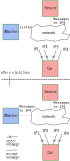
\includegraphics[width=0.3\textwidth]{schema/new2.pdf}
    \caption{Illustration of the proposed pool-based address switching scheme}
    \label{second}
\end{figure}

\subsection{ Example}

Figure \ref{second} illustrates a manufacturer's subnetwork, with a
connected car equipped with four network interfaces with each one an
IP address assigned, \emph{IP1}, \emph{IP2}, \emph{IP3}, and \emph{IP4}, as well as an
external service and an attacker connected to the subnetwork. In the
beginning, \emph{IP4} is the active IP address that accepts incoming
messages, while the other three reject all incoming messages. The car
communicates with the service, which responds by sending messages to
\emph{IP4}. Since the IP address of the car is visible in the header of any
circulating message in the network, the attacker can discover the IP
address of the car and may try to communicate with the car via
\emph{IP4}. Once the active time period of \emph{IP4} ends (after $x \in [a,b]$
time units), the DHCP server elects the new IP address accepting
messages, and sends -- in an encrypted message -- the new
configuration to the car. As shown in the lower part of the figure,
\emph{IP2} now becomes the active address, while \emph{IP4} will drop any
incoming messages.


\subsection{Protection}

If the attacker launches the attack before the currently receiving IP
address expires, he or she can start to communicate with the
discovered car. If the valid time period per IP address is short
enough, the address switch will take place before the attacker can
complete a successful attack. Assuming that an entire fleet of
vehicles is equipped with the proposed MTD mechanism, a massive
parallel attack against the whole fleet will be impractical: if the
attacker assembles a hit-list of collected IP addresses, these will
likely have changed at the time the attack starts. Since the
assignment of the receiving IP addresses and their active time window
is sent encrypted, the attacker will not be able to learn which
address the car has switched to once the currently active interface
stops responding.


As a conclusion, changing the IP address slows down an attacker coming
from inside of the subnetwork. This attacker will see the IP addresses
of the different cars communicating on the subnetwork. If he or she is
seeking to retrieve information about one discovered car before
launching his or her attack, he or she may even not be able to launch
his or her attack at all. By periodically changing the address, this
makes the time available for an attacker to perform his or her attack
shorter than without this mechanism.

\subsection{Cost} 

The presented defense mechanism can easily be implemented on top of an
existing network. It does not entail major infrastructure changes nor
heavy network trafic overhead. To apply this method in an existing
system, it will be necessary to setup *MPTCP* on the side of the
vehicles. Furthermore, it requires adding $N$ new physical network
interfaces on each car and adapting the car's firewall rules. On the
side of the network infrastructure, it will be necessary to slightly
modify the DHCP server for each subnetwork in order to implement the
assignment of an address pool to each newly connecting car and the
address renewal mechanism choosing a new address from the pool.

\subsection{ Discussion} 

It can be argued that the addition of several IP address would
facilitate the discovery of a fleet of vehicle from outside the
network, and this is actually the case.  The time to reach a 50\%
probability of finding one of the IP address is $3 \cdot 10^{12}$ s,
or 95 years instead of 951.  This remains a very acceptable
time. Especially since when an attacker succeeds in finding one of the
vehicles, there is only a $1/N$ chance that this IP address is the
active IP address that receives the messages.


This technique is able to repel attackers even from inside the network
if the period of IP address change is sufficiently small. However,
there remains a risk of \emph{Denial of Service} (DoS) attacks. This
vulnerability is due to the fact that each car is assigned a
\emph{static} address pool from the beginning to the end of its
connection on the network. This means that the addresses from this
pool will be used several times as the accepting address for incoming
messages.  This periodic re-use of the same addresses allows an
attacker to establish a list of known addresses and to flood them with
messages continuously, resulting in a denial of service. Therefore, an
alternative approach -- which will be presented in the following --
limits address reuse.

\section{Randomized Pool-based IP Address Switches}

\label{sec:second}

{\Huge I}n this section, we describe an alternative MTD approach that
additionally aims to protect the connected vehicles against DoS
attacks, while trying to limit the impact on the network
infrastructure. We keep the same assumptions about the system: all
cars of the same manufacturer are connected to the same IPv6
subnetwork controlled by the manufacturer; each car has $N$ network
interfaces providing it with $N$ IP addresses on this
network. Likewise, we are still using MPTCP to maintain several open
connection paths as well as the periodic change of the IP address
accepting messages. However, we make the address pool associated with
each car dynamic, i.e. addresses will change over time, such that no
address will be used twice by the same car, in order to avoid DoS.


\subsection{Approach principle}


As before, at the first connection of a car on a network, the DHCP
server assigns an IP address to each of its interfaces and indicates
the interface that will accept incoming messages.

However, in addition to regularly switching the active interface of
each car, the DHCP server will send an encrypted message, ordering the
receiving car to replace the IP address of one of the \emph{inactive}
interfaces with a fresh one. The car needs to do the necessary changes
in its configuration, and update the corresponding interface to use
the new address once it will become the active interface. This implies
also adding the new address to the MPTCP rules as a new route to the
car. In order to avoid packet loss, and give the car sufficient time
for reconfiguration, the address change occurs \emph{in the
background}, \emph{i.e.} it never affects the currently active interface and
does not interfere with the car's communication.

The period by which new addresses will be assigned can be chosen freely, leading
to different trade-offs of costs and security. If it is longer than the validity
period, this will lead to address reuse. By always renewing the address of the
least recently deactivated interface, the address pool of size N is completely
renewed every N address changes. As a consequence, no address will ever be
active twice\footnote{unless the same address is randomly chosen twice by the
DHCP server, which has a sufficiently low probability.}, as illustrated by the
following example.

\begin{figure}[h]
    \centering
	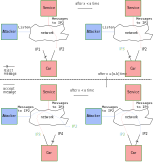
\includegraphics[width=0.6\textwidth]{schema/new4.pdf}
    \caption{Illustration of the randomized pool-based address switching with 2 network interfaces per vehicle}
    \label{third}
\end{figure}

\subsection{ Example}

Figure \ref{third} shows the randomized address switching for the case
$N=2$, i.e. each car has two network interfaces. The car *Car* is
connected to the manufacturer's subnetwork and has currently addresses
IP1 and IP2 assigned to its interfaces, where IP2 is the address
accepting incoming messages. the \emph{Car} communicates with a service on
the network, while an attacker listens to the network
traffic. Meanwhile the *Car* receives instructions from the server to
replace the address IP1 with the fresh address IP3, so it updates its
interfaces, MPTCP rules and firewall rules. Once the valid time period
of IP2 expires, IP3 becomes the active address accepting incoming
messages, while the attacker still tries to communicate via IP2. The
*Car* continues its communication with the service while the
attacker's messages are rejected on IP2. Meanwhile, the car then
receives instructions to change IP2 to IP4, so the attacker now talks
to an unknown address. By changing addresses at each time period, the
attacker only has this period to launch his or her attack and can no
longer anticipate changes in the \emph{Car's} addresses.

\subsection{Costs}

If the address renewal period is equal to the validity period -- as in
the above example -- each address is only used once. Thus, there is no
need to choose $N$ greater than two, as this does not increase the
entropy. Therefore, the constant costs related to the number of
network interfaces are lower than in the static pool-based approach
with $N > 2$. However, there is an additional overhead for the network
infrastructure: firstly, there are additional address renewal messages
sent out by the DHCP server. Secondly, the DHCP server itself has
additional work to do choosing new addresses and changing its internal
routing tables.

\subsection{Randomization on Demand}

An alternative application of the randomized address-renewal would be
to use it in addition to the first method. In other words, equipping
the cars with $N$ network interfaces with addresses assigned per
interface that do not automatically change over time. But when a
persistent attack on the network is discovered, an address renewal is
triggered: for the list of vehicles under attack, the pool of
available addresses is updated, thus preventing denial of service.


\begin{figure}[h]
    \centering
	\includegraphics[width=0.65\textwidth]{schema/new3.pdf}
    \caption{illustration of the method with N network interfaces per vehicle}
    \label{Random1}
\end{figure}

Figure \ref{Random1} illustrates this
combined approach. There is a car connected to the subnetwork with 4
network interfaces, corresponding to the IP addresses IP1, IP2, IP3,
and IP4. In the beginning, IP4 is the only address accepting incoming
messages. As before, an attacker is listening to messages circulating
on the network. Upon detection of the intruder, the car receives
instructions from the DHCP server to change IP2 address to IP5, and it
updates the MPTCP and firewall rules. At the end of the validity
period IP5 becomes the new accepting address.  The attacker will try
to attack IP4 which no longer accepts incoming messages.  In contrast,
in the absence of a detectable threat, the address pool will remain
stable, avoiding additional network traffic and server load.

\subsection{Discussion} 

By adding randomized renewal, DoS attacks can be thwarted, with higher
costs incurred by network traffic overhead and increased DHCP server
load. Between the two extremes -- no address renewal at all or after
each interface swap -- the renewal period can be chosen in order to
adapt the overhead and the security level to the use case and
available infrastructure. As an alternative, addresses can be renewed
on demand only, in combination with an appropriate attack detection
mechanism.



\section{Conclusion}

\label{sec:con}

{\Huge I}n this paper, we investigate a moving target defense in the context of
connected objects on an IPv6 network. In particular, we consider connected cars
sharing a common manufacturer's subnetwork, which makes them particularly
vulnerable to attacks from within the same network. 

As a remedy, we propose a dynamic address switching scheme relying on the
network's DHCP server. In our approach, each connected car disposes of several
redundant network interfaces, each with a separate IP address. This allows for
dynamic address switching without connection losses. The basic protection
mechanism is that each car only accepts incoming messages on one interface at
any time, leaving attackers talking to inactive addresses after a switch. While
the basic approach uses fixed address pools, an additional address renewal by
the DHCP server can help to thwart denial of service attacks, since it allows to
avoid address reuse. Adjusting both the periods for address switching and
address renewal leads to a flexible MTD approach that can be adapted to the
security requirements and network infrastructure at hand. To the best of our
knowledge, this is the first network MTD approach presented in the context of an
IPv6 subnetwork which considers attacks from within the same network.

